\FILE{cloudmesh.tex}

\section{Cloudmesh\footnote{This section is als available in part from
  the cloudmesh Web pages and includes large protions of copied
  text. The text is publically available.}}\label{S:cloudmesh}

From the experience with FutureGrid we identified the need for a more
tightly integrated software infrastructure addressing the need to
deliver a software-defined system – encompassing virtualized and
bare-metal infrastructure, networks, application, systems and platform
software – with a unifying goal of providing Cloud Testbeds as a
Service (CTaaS). This system is termed cloudmesh to symbolize (a) the
creation of a tightly integrated mesh of services targeting multiple
IaaS farmeworks (b) the ability to federate a number of resources from
from academia and industry. This includes existing FutureGrid
infrastructure, Amazon Web Services, Azure, HP Cloud, Karlsruhe using
not only one IaaS framework but various. (c) The creation of an
environment in which it becomes more easy to experiment with platforms
and softwere services while assiting to deploy them more easily.
In addition to virtual resources, FutureGrid exposes bare-metal
provisioning to users, but also a subset of HPC monitoring
infrastructure tools. Services will be available through command line,
API, and Web interfaces.

\subsection{Functionality}

Cloudmesh provides due to its integrated services the ability to be an
onramp for other clouds. It also provides information services to
various system level sensors to give access to sensor and utilization
data. They internally can be used to optimize the system
usage. The provisioning experience from FutureGrid has taught us that
we need to provide the creation of new clouds, the repartitioning of
resources between services (cloud shifting), and the integration of
external cloud resources in case of over provisioning (cloud
bursting). As we deal with many IaaS we need an abstraction layer on
top of the IaaS framework. Experiment management is conducted with
workflows controoled in shells, Python/iPython, as well as systems
such as Heat, Accounting is supported through additional services such
as user management and charge rate management. Not all features are
yet implemented. Figure \label{F:cm-func} shows the main functionality
that we target at this time to implement.

\begin{figure}[h!]
  \centering
    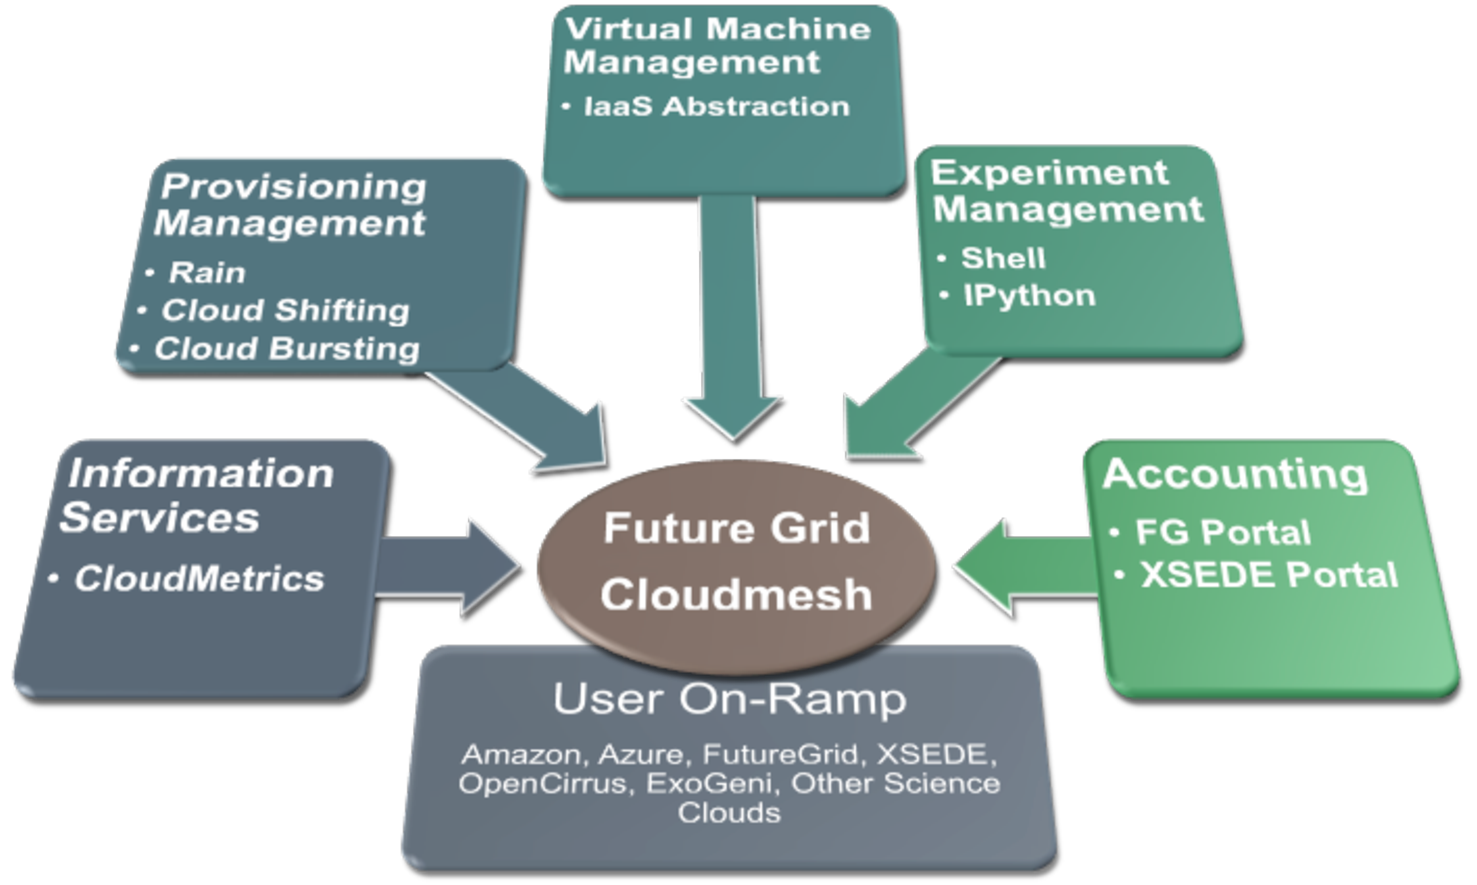
\includegraphics[width=1.0\textwidth]{images/cm-functionality.pdf}
  \caption{CM Functionality.}\label{F:cm-func}
\end{figure}


\subsection{Architecture}

The three layers of the Cloudmesh architecture include a Cloudmesh
Management Framework for monitoring and operations, user and project
management, experiment planning and deployment of services needed by
an experiment, provisioning and execution environments to be deployed
on resources to (or interfaced with) enable experiment management, and
resources.

\begin{figure}[h!]
  \centering
    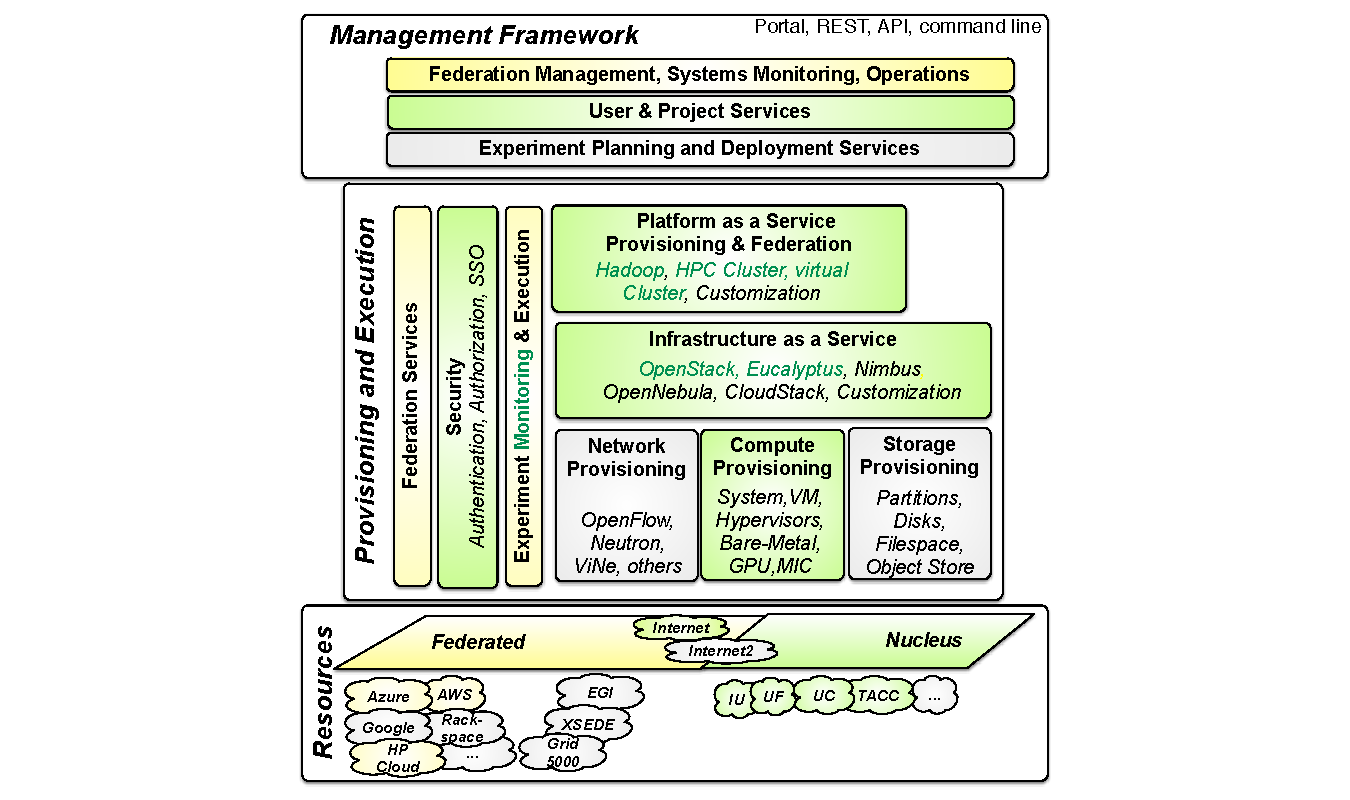
\includegraphics[width=1.0\textwidth]{images/cm-arch.pdf}
  \caption{CM Architecture.}
\end{figure}

\paragraph{System Monitoring and Operations.}

The management framework contains services to facilitate FutureGrid day-to-day operation, including federated or selective monitoring of the infrastructure. Cloudmesh leverages FutureGrid for the operational services and allows administrators to view ongoing system status and experiments, as well as interact with users through ticket systems and messaging queues to inform subscribed users on the status of the system.
The cloudmesh management framework offers services that simplify integration of resources in the FutureGrid nucleus or through federation. This includes, for user management, access to predefined setup templates for services in enabling resource and service provisioning as well as experiment execution. To integrate IaaS frameworks cloudmesh offers two distinct services:

(a) a federated IaaS frameworks hosted on FutureGrid,
(b) the availability of a service that is hosted on FutureGrid allowing the “integration” of IaaS frameworks through user credentials either registered by the users or automatically obtained from our distributed user directory.

For (b) several toolkits exist to create user-based federations, including our own abstraction level which supports interoperability via libcloud, but more importantly it supports directly the native OpenStack protocol and overcomes limitations of the EC2 protocol and the libcloud compatibility layer. Plugins that we currently develop will enable access to clouds via firewall penetration, abstraction layers for clouds with few public IP addresses and integration with new services such as OpenStack Heat. We successfully federated resources from Azure, AWS, the HP cloud, Karlsruhe Institute of Technology Cloud, and four FutureGrid clouds using various versions of OpenStack and Eucalyptus. The same will be done for OpenCirrus resources at GT and CMU through firewalls or proxy servers.
Additional management flexibility will be introduced through automatic cloud-bursting and shifting services. While cloud bursting will locate empty resources in other clouds, cloud shifting will identify unused services and resources, shut them down and provision them with services that are requested by the users. We have demonstrated this concept in 2012, moving resources for ~100 users to services that were needed based on class schedules. A reservation system will be used to allow for reserved creation of such environments, along with improvements of automation of cloud-shifting.

\paragraph{User and Project Services}

FutureGrid user and project services simplify the application processes needed to obtain user accounts and projects. We have demonstrated in FutureGrid the ability to create accounts in a very short time, including vetting projects and users – allowing fast turn-around times for the majority of FutureGrid projects with an initial startup allocation. Cloudmesh re-uses this infrastructure and also allows users to manage proxy accounts to federate to other IaaS services to provide an easy interface to integrate them.

\paragraph{Accounting and App Store}

To lower the barrier of entry Cloudmesh will be providing a shopping cart which will allow checking out of predefined repeatable experiment templates. A cost is associated with an experiment making it possible to engage in careful planning and to save time by reusing previous experiments. Additionally, the Cloudmesh App Store may function as a clearing-house of images, image templates, services offered and provisioning templates. Users may package complex deployment descriptions in an easy parameter/form-based interface and other users may be able to replicate the specified setup with.
Due to our advanced Cloudmesh Metrics framework we are in the position to further develop an integrated accounting framework allowing a usage cost model for users and management to identify the real impact of an experiment on resources. This will be useful to avoid overprovisioning and inefficient resource usage. The cost model will be based not only on number of core hours used, but also the capabilities of the resource, the time, and special support it takes to set up the experiment. We will expand upon the metrics framework of FutureGrid that allows measuring of VM and HPC usage and associate this with cost models. Benchmarks will be used to normalize the charge models.

\paragraph{Networking.}

We have a broad vision of resource integration in FutureGrid with systems offering different levels of control from “bare metal” to use of a portion of a resource. Likewise, we must utilize networks offering various levels of control, from standard IP connectivity to completely configurable SDNs as novel cloud architectures will almost certainly leverage NaaS and SDN alongside system software and middleware. FutureGrid resources will make use of SDN using OpenFlow whenever possible and the same level of networking control will not be available in every location.

\paragraph{Monitoring.}

To serve the purposes of CISE researchers, Cloudmesh must be able to access empirical data about the properties and performance of the underlying infrastructure beyond what is available from commercial cloud environments. To accommodate this requirement we have developed a uniform access interface to virtual machine monitoring information available for OpenStack, Eucalyptus, and Nimbus. In the future, we will be enhancing the access to historical user information. Right now they are exposed through predefined reports that we create on a regular basis. To achieve this we will also leverage the ongoing work while using the AMPQ protocol. Furthermore, Cloudmesh will provide access to common monitoring infrastructure as provided by Ganglia, Nagios, Inca, perfSonar, PAPI and others.

\begin{figure}[h!]
  \centering
    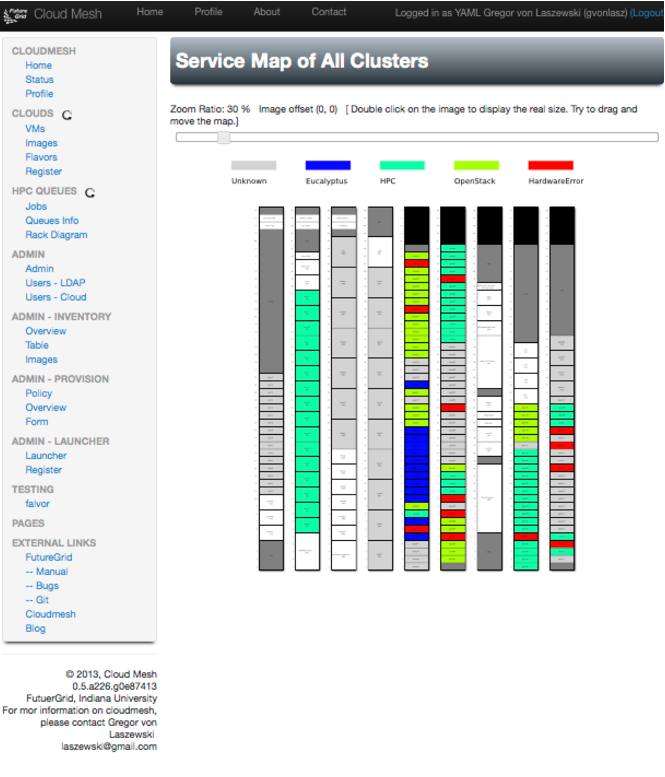
\includegraphics[width=.7\textwidth]{images/rainbow.pdf}
  \caption{Monitoring the Service distribution of FutureGrid with cloudmesh.}
\end{figure}

\subsection{Cloud Shifting}

We have already demonstrated via the RAIN tool in cloudmesh that it is
possible to easily shift resources between services. We are currently
expanding upon this idea and developing more easy to use user
interfaces that assit administrators and users through role and
project based authentication to move resources from one service to
another (see Figure \ref{F:shift}).

\begin{figure}[h!]
  \centering
    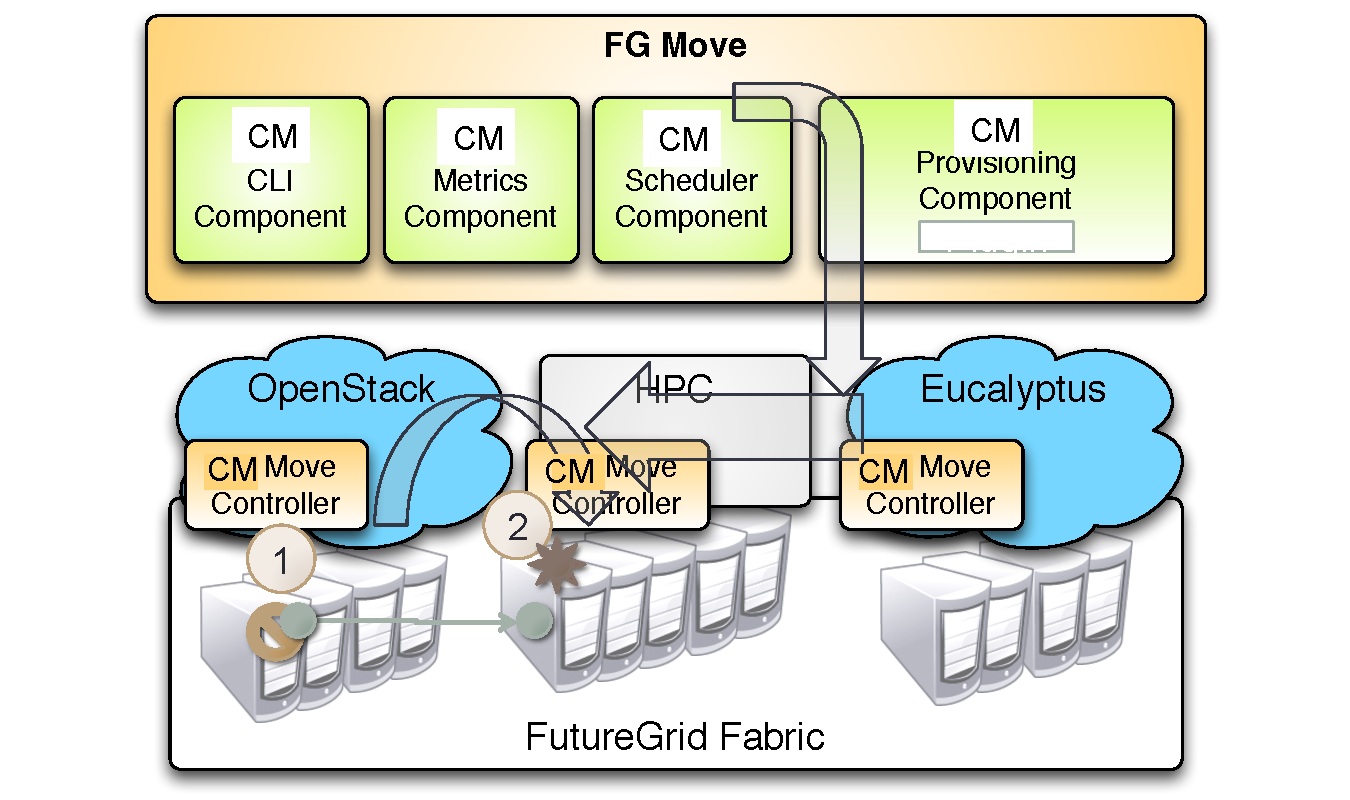
\includegraphics[width=1.0\textwidth]{images/shift2.pdf}
  \caption{Shifting resources makes it possible to offer flexibility
    in the service distribution in case of over or underprovisioning.}\label{F:shift}
\end{figure}

\subsection{Graphical User Interface}

Despite the fact that cloudmesh was originally a quite sophisticated
command shell and commandline tool, we have spend recently more time
in exposing this functionality through a conveneient Web
interface. Some mor popular views if this interface are depicted in
Figure \ref{F:instances} hinting on how easy it is with a single
button to create multiple VMs accross a variety of IaaS. Also nice is
that this not only includes resources at IU but also at external
locations. Pushing this easy management in a more sophisticated
experience for the user while associating one-click deployments that
include the ability to deploy virtual clusters, hadoop environments,
and other more elaborate setups wie provide an early prototype
screenshot in Figure \ref{F:oneclick}.

\begin{figure}[htb]
  \centering
    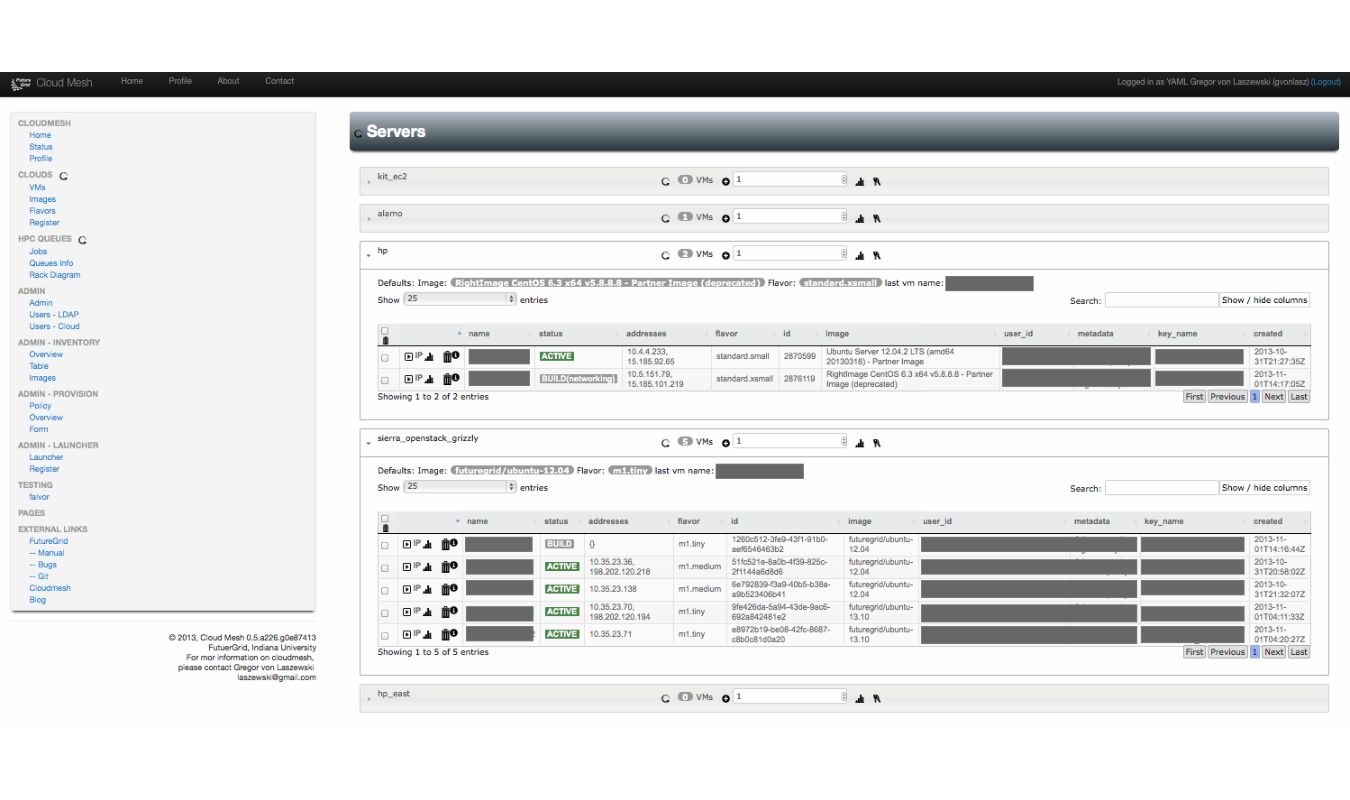
\includegraphics[width=.9\textwidth]{images/instances.pdf}
  \caption{Rainbow.}\label{F:instances}
  \centering
    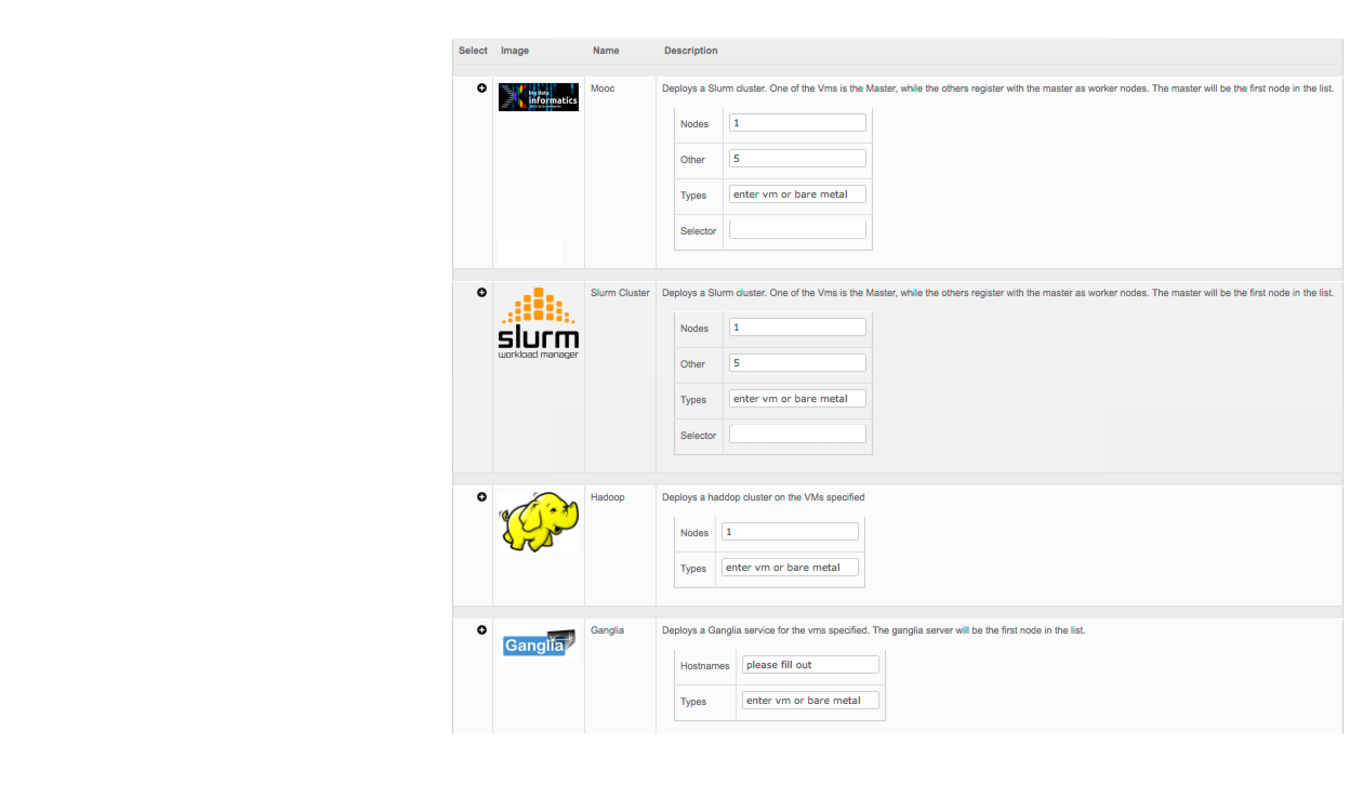
\includegraphics[width=.9\textwidth]{images/oneclick.pdf}
  \caption{One click deployment of platforms and sophisticated
    services that could even spawn multiple resources.}\label{F:oneclick}
\end{figure}


\afterpage{\clearpage}